\section{Vídeo}
\begin{frame}[allowframebreaks]
  \frametitle{Vídeo}
  \vspace{-2ex}
  \begin{figure}[h]
  \centering
  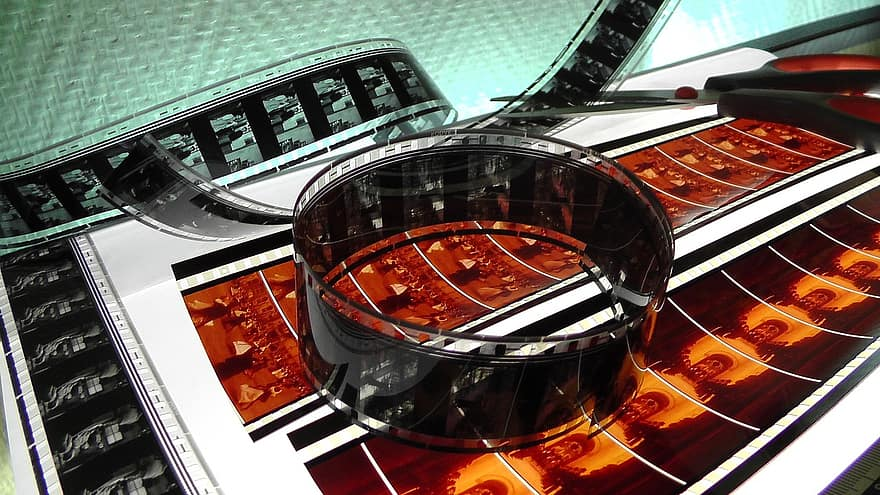
\includegraphics[width=0.4\textwidth]{images/film70mm.jpg}
  \caption{Película de 70mm (pikist.com).}
  \label{fig:film70mm}
  \end{figure}
  \vspace{-2ex}
  \begin{figure}[h]
  \centering
  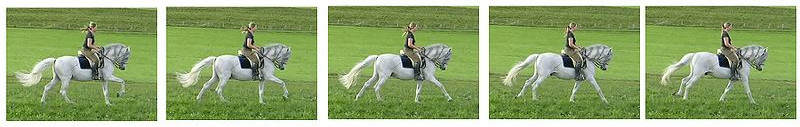
\includegraphics[width=0.6\textwidth]{images/motion.jpg}
  \caption{Movimento (Wikipedia).}
  \label{fig:motion}
  \end{figure}
\end{frame}
\note{
Sequência de quadros exibidos em sucessivamente a uma determinada taxa: quadros por segundo (FPS, \textit{frames per second}),
uma unidade de medida da cadência de um dispositivo.

``The human visual system can process 10 to 12 images per second and perceive them individually, while higher rates are perceived as motion.''
\url{https://en.wikipedia.org/wiki/Frame_rate}

}


\begin{frame}[allowframebreaks]
  \frametitle{Codificação de vídeo}
  \bibentry{zeng2013}

  \begin{figure}[h]
  \centering
  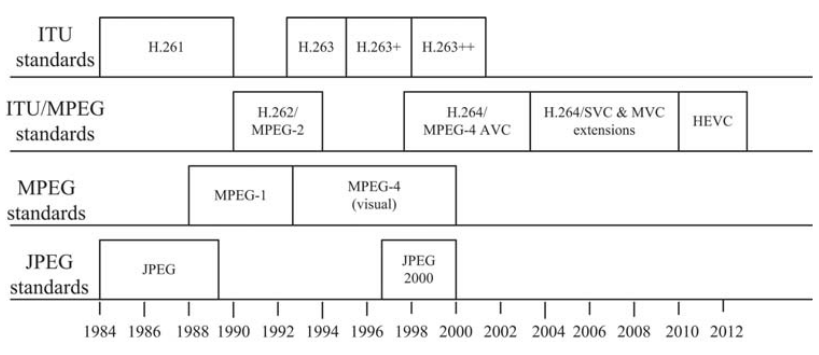
\includegraphics[width=0.6\textwidth]{images/videocodectimeline.png}
  \caption{Linha do tempo dos padrões de codificação de imagem e vídeo \citep{zeng2013}.}
  \label{fig:videocodectimeline}
  \end{figure}

  \framebreak

  \begin{figure}[h]
  \centering
  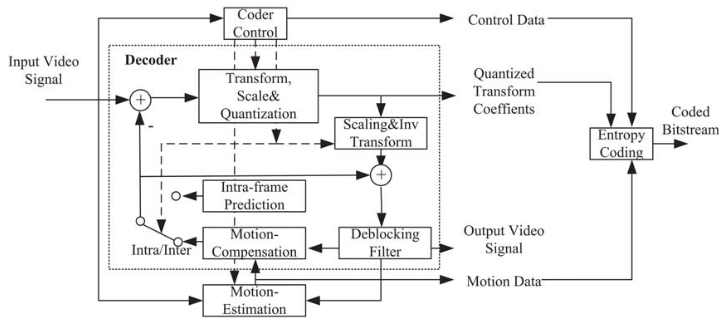
\includegraphics[width=0.75\textwidth]{images/videocodingschema.png}
  \caption{Estrutura genérica de um codificador de vídeo \citep{zeng2013}.}
  \label{fig:videocodingschema}
  \end{figure}

\end{frame}
\note{
  Padronização:
  \begin{itemize}
  \item interoperabilidade
  \item suporte a aplicações existentes e futuras
  \item diferentes implementações
  \end{itemize}
}
\note{
  Elementos básicos da compressão de vídeo:
  \begin{itemize}
  \item predição temporal: explorar a redundância entre quadros
  \item transformada - decomposição no domínio da frequência: aplicar a DCT
          em blocos para explorar as característica estatísticas e perceptuais 
          da redundância na informação espacial
  \item quantização: redução de precisão seletiva para minimizar o \textit{bit rate} sem
          gerar degradação perceptiva da qualidade
  \item codificação de entropia: explorar a redundância estatística em um sequência de símbolos 
          dos dados provenientes da quantização e das informações complementares
  \end{itemize}
}
\note{
Em um vídeo, temos longas sequências de quadros em que um mesmo objeto (ou fundo) aparece continuamente (parado ou em movimento).
A estimação de movimento é utilizada para examinar o movimento de objetos em uma sequência de imagens, buscando obter
vetores que representem o movimento estimado.
A compensação de movimento utilizado o conhecimento da movimentação de objetos para obter compressão dos dados.
Na codificação inter quadro\footnote{
O inter quadro (\textit{inter frame}), em uma sequência de quadros de um vídeo, é um quadro expresso em função de outros quadros vizinhos.
}, a estimação e compensação de movimento são técnicas importantes para remover a redundância temporal
devido à grande correlação existente entre quadros sucessivos, permitindo que uma alta taxa de compressão seja obtida.
}
\note{
É usual utilizar o espaço de cores YCbCr, separando informação de luminância e crominância.
A degradação de informação de crominância é menos perceptível. Por este motivo faz-se uso 
da subamostragem de crominância.

\url{http://en.wikipedia.org/wiki/Chroma_subsampling}
}
\note{
Um requisito importante na codificação de vídeo é garantir o acesso aleatório, ou seja,
permitir a codificação de um vídeo a partir e um instante qualquer (ou próximo).
}
\note{
Quandros em uma sequência são preditos a partir de outros quatros na sequência.
Uma consequência negativa é que error gerados são propagados em todos os quadros interdependentes.
Para amenizar este efeito, utiliza-se o \textit{refresh}, enviando periodicamente 
um quadro completo, sem o uso de predição, permitindo assim que o decodificador ressincronize
a partir daquele ponto.

Outra técnica utilizada é o \textit{leaky prediction}, uma taxa de `esquecimento' no preditor para que perturbações não se propagem 
ao longo de vários quadros. Esta piora intencional do preditor fará com que mais informação
componha o erro de predição.
}



\begin{frame}[allowframebreaks]
  \frametitle{Tipos de quadros}

  Tipos de quadros:
  \begin{description}
  \item[I frame] - quadros `Intra-codificados'' (quadros chaves, \textit{key frames})
  \item[P frame] - quadros preditos  %predicted based on prior I or P frames plus the addition of data for changed macroblocks.
  \item[B frame] - quadros preditos bidirecionais %based on appearance and positions of past and future frames macroblocks.
  \end{description}

  \begin{figure}[h]
  \centering
  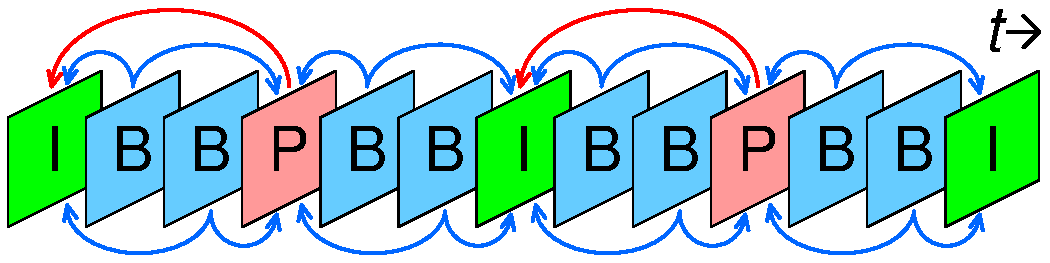
\includegraphics[width=0.75\textwidth]{images/interframegroup.pdf}
  \caption{Sequência de quadros (Wikipedia).}
  \label{fig:interframegroup}
  \end{figure}


\end{frame} 
